Eine Aussage über die Energieauflösung ist erst möglich, wenn sowohl das Rauschen als auch die Form des Signals bekannt sind.
Für die Bestimmung der Energieauflösung ist es also notwendig einen Beispielsignal, wie wir es erwarten würden, zu bestimmen.
Wie in den Kapiteln \ref{sec:Entstehung} und \ref{sec:Elektronik} gezeigt erzeugt ein Event, welches die Energie $E$ deponiert, eine bestimmte Zahl Elektron-Loch-Paare $N_{eh}$ abhängig von einer materialspezifischen mittleren Energie zur Erzeugung eines Elektron-Loch-Paars $\epsilon$.
Für den Strom der durch ein solches Event in der Elektronik induziert wird, ergibt sich somit entsprechend Gleichung \eqref{eq:RamoCharge}
\begin{equation}
I_{sig}(t) = e\frac{E}{\epsilon}(a-b)\delta (t).
\end{equation}
Durch die Transformation in den Frequenzraum und Multiplikation mit der Eingangsimpedanz erhalten wir das eingangsseitige Spektrum des Signals
\begin{equation}
s(f) = e\frac{E}{\epsilon}(a-b)\frac{1}{2\pi f C_{ges}}.
\end{equation}
Das Bestimmen der Energieauflösung wird mittels der Optimal Filtering Methode(siehe Anhang \ref{sec:OpFiltering}) durchgeführt und ist gegeben durch
\begin{equation}
\sigma^2_E = \frac{N}{f_s}\left(4\sum_{n=0}^{N/2}\frac{|s(f_n)|^2}{J_{ss}(f_n)}\right)^{-1}
\label{eq:OptFilt}
\end{equation}
$J_{ss}$ die spektrale Leistungsdichte für $f>0$, $N$ die Anzahl von Datenpunkten und $f_s$ die Samplerate.

Aus dieser Gleichung lässt sich erkennen, dass die Verstärkung keinen Einfluss auf die Auflösung hat, da sowohl das Signal $s(f)$ als auch das Rauschen $J_{ss}$ gleichermaßen verstärkt werden.
Die Verstärkung muss nur groß genug sein, sodass das Rauschen der nachfolgenden Elektronik keine Rolle spielt.
Auf diese Weise wurde für das in Abb. \ref{fig:54ROpen} gezeigte Rauschen die in Abb. \ref{fig:Resolution} gezeigte Energieauflösung bestimmt.
Für das Signal $s(f)$ sind unterschiedliche Eingangskapazitäten angenommen worden.
Da das Rauschen bei immer der gleichen Eingangskapazität von $C_{ges}=\SI{104,25}{\pico\farad}$ aufgenommen wurde, entspricht die Energieauflösung nur bei gleicher Eingangskapazität von Signal und Rauschen der realen Situation (in Abb. \ref{fig:Resolution} gestrichelt dargestellt).
Oberhalb (unterhalb) der gestrichelten Linie ist die dargestellte Energieauflösung minimal größer (kleiner) als die reale, da das Rauschen der Rauschstromquelle mit der Eingangsimpedanz kleiner(größer) wird.
Um die Elektronik mit der anderer Experimente zu vergleichen, welche Detektoren mit größeren Kapazitäten verwenden, ist diese Darstellung gewählt worden.

\begin{figure}[!t]
\begin{center}
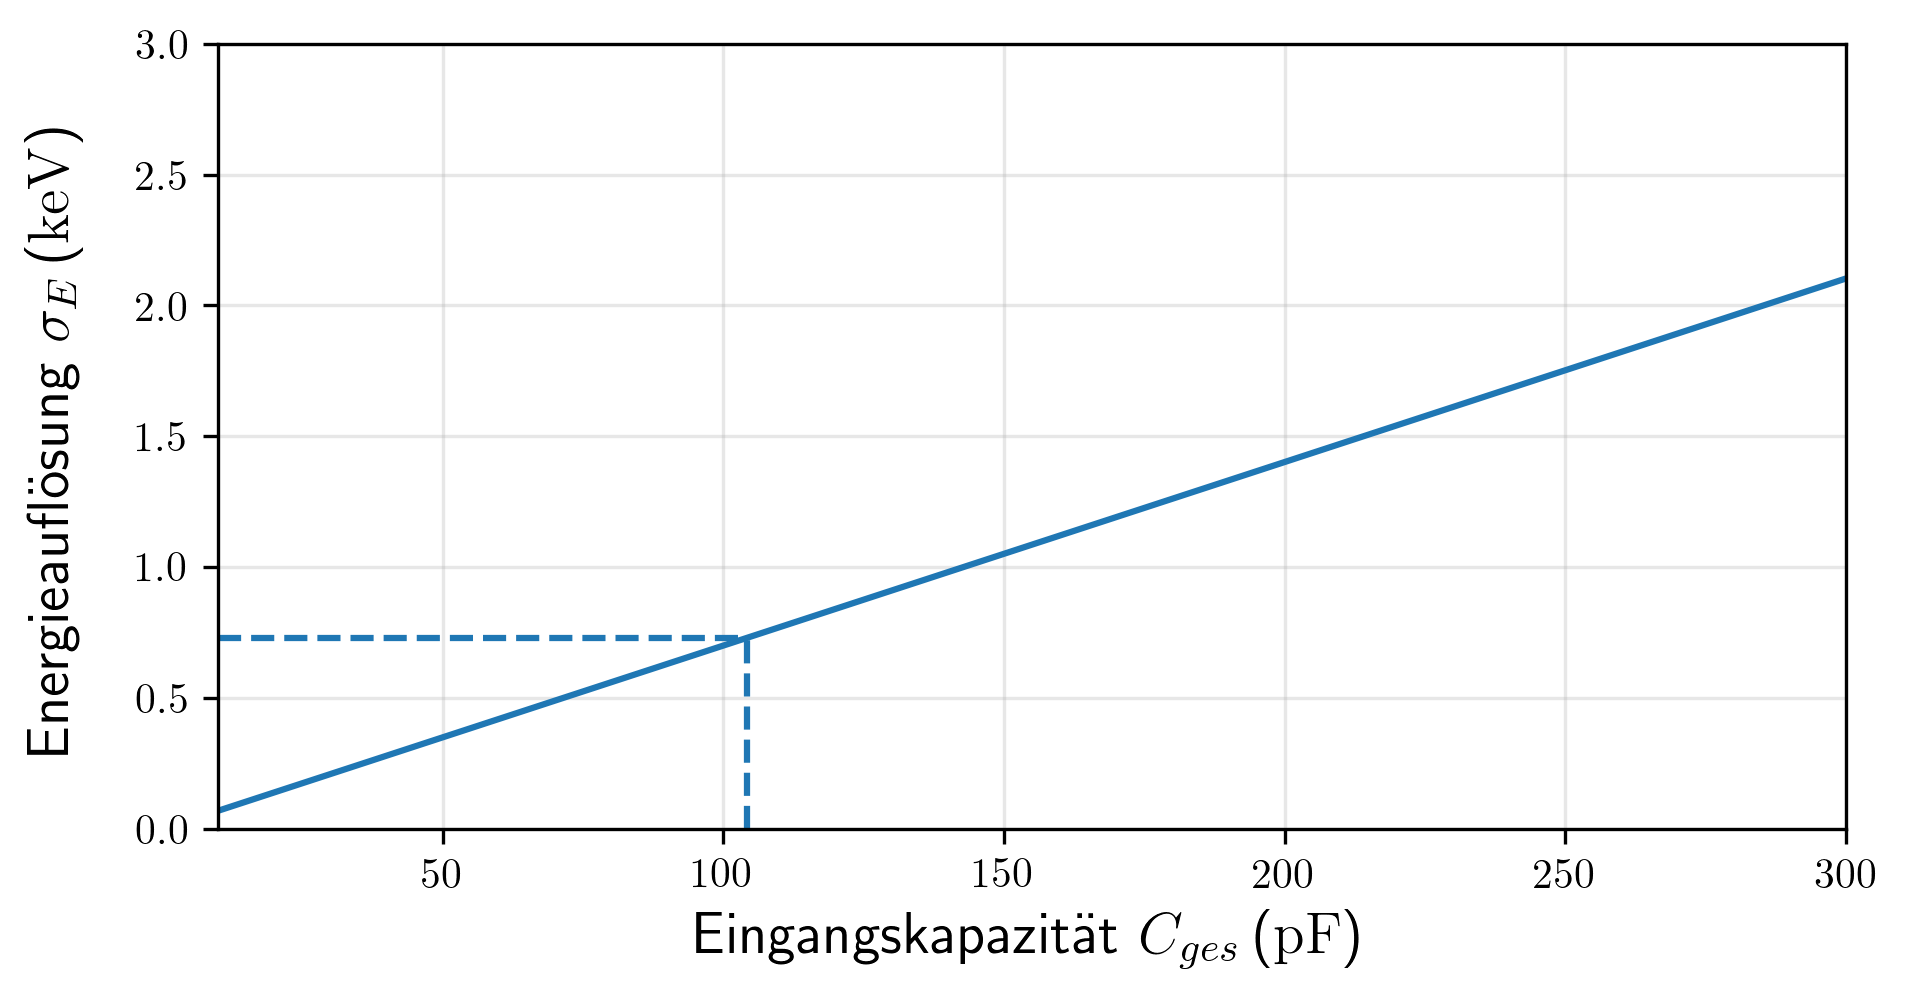
\includegraphics[width=\textwidth]{./fig/Resolution.png}
\vspace{-0.5cm}
\caption{Energieauflösung wenn $100\%$ des Angelegten Potentials von den Ladungsträgern Durchlaufen wird in Abhängigkeit der Eingangskapazität.
Berechnet gemäß Gl. \eqref{eq:OptFilt} aus dem in Abb. \ref{fig:54ROpen} gezeigten Rauschen der kalten Elektronik.
Das Rauschen wurde bei der Gesamtkapazität von $C_{ges}=\SI{104,25}{\pico\farad}$ aufgenommen.
Die gestrichelten Linien zeigen die Energieauflösung, wenn die Gesamtkapazität zur Berechnung des Signals $s(f)$ gleich der Gesamtkapazität der kalten Elektronik ist.}
\label{fig:Resolution}
\end{center}
\end{figure}

Bei einer Kapazität von $C_{ges}=\SI{104,25}{\pico\farad}$ ist die Energieauflösung $\sigma_E = 1/(a-b)\cdot \SI{0,731}{\kilo\electronvolt}$.
Die Energieauflösung ist abhängig von dem Prozentsatz des der Ladungsträger durchlaufenen Potentials $a-b$.
In dem Aufbau der EDELWEISS oder CDMS Elektrode durchlaufen die Ladungsträger $100\%$ des angelegten Potentials ($a-b=1$) da die Elektroden unmittelbar auf dem Detektor aufgedampft sind.

In Abbildung \ref{fig:EDWIII} ist die spektrale Leistungsdichte des EDELWEISS-III Ionisationskanals bei $\SI{4}{\kelvin}$ mit einem auf $\SI{100}{\kelvin}$ geheiztem JFET dargestellt.
Damit wurde eine Energieauflösung von $\SI{212}{\electronvolt}$ erreicht\cite{EDWIII} unter Verwendung eines $\SI{150}{\pico\farad}$ Detektor mit zusätzlich $\SI{100}{\pico\farad}$ Kapazität durch die Kabel und $\SI{50}{\pico\farad}$ Eingangskapazität des JFET.
Die beste von Axel Gullasch erreichte Energieauflösung mit der gleichen Elektronik ist $\SI{2.11}{\kilo\electronvolt}$ bei einer Temperatur von $\SI{200}{\kelvin}$\cite{Gullasch2015}.
Allerdings ohne Angabe der Eingangskapazität.

Mit CNRS HEMTs ist eine Energieauflösung von $\SI{91}{\electronvolt}$ mit einem $\SI{150}{\pico\farad}$ CDMS-Detektor gelungen \cite{Phipps2016}.

\begin{figure}[!b]
\begin{center}
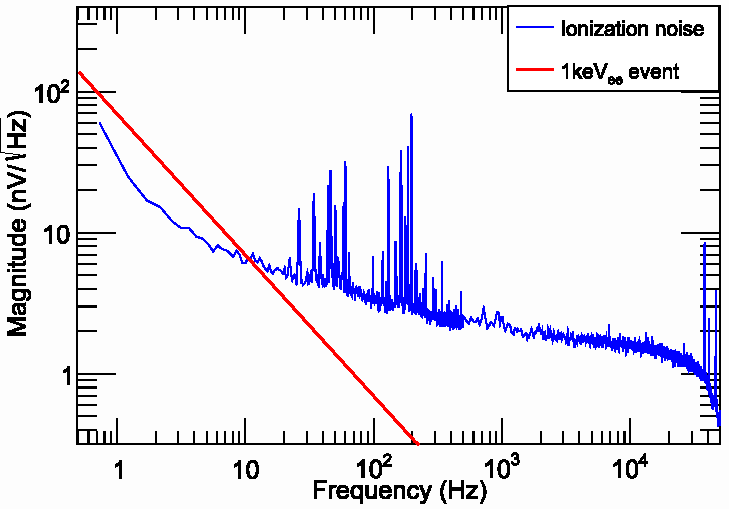
\includegraphics[width=\textwidth]{./fig/Rauschen/EDWIIIPerformance.pdf}
\vspace{-0.5cm}
\caption{Spektrale Leistungsdichte des JFET basierten EDELWEISS-III Ionisationskanals bei $\SI{4}{\kelvin}$.
Der JFET wird auf $\SI{100}{\kelvin}$ geheizt.
Bei einer Eingangskapazität von \SI{300}{\pico\farad} zusammengesetzt aus \SI{150}{\pico\farad} Detektorkapazität, \SI{100}{\pico\farad} Kapazität der Kabel und \SI{50}{\pico\farad} Kapazität des JFET.
Das Spektrum eines erwarteten $\SI{1}{\kilo\electronvolt}$ Signalpuls ist in rot dargestellt.\cite{EDWIII}}
\label{fig:EDWIII}
\end{center}
\end{figure}
